\documentclass{article}

% use Times
\usepackage{times}
% For figures
\usepackage{graphicx} % more modern
\usepackage{subfigure} 
\usepackage{amsmath,amssymb,amsthm} 

% For citations
\usepackage{natbib}

% For algorithms
\usepackage{algorithm}
\usepackage{algorithmic}

% As of 2011, we use the hyperref package to produce hyperlinks in the
% resulting PDF.  If this breaks your system, please commend out the
% following usepackage line and replace \usepackage{icml2014} with
% \usepackage[nohyperref]{icml2014} above.
\usepackage{hyperref}

% Packages hyperref and algorithmic misbehave sometimes.  We can fix
% this with the following command.
\newcommand{\theHalgorithm}{\arabic{algorithm}}

% Employ the following version of the ``usepackage'' statement for
% submitting the draft version of the paper for review.  This will set
% the note in the first column to ``Under review.  Do not distribute.''
\usepackage{icml2014} 
% Employ this version of the ``usepackage'' statement after the paper has
% been accepted, when creating the final version.  This will set the
% note in the first column to ``Proceedings of the...''
%\usepackage[accepted]{icml2014}


% The \icmltitle you define below is probably too long as a header.
% Therefore, a short form for the running title is supplied here:
%\icmltitlerunning{Submission and Formatting Instructions for ICML 2014}

% Text
\newcommand{\todo}[1]{\hl{\textbf{TODO:} #1}}
\newcommand{\citationneeded} {\ensuremath{^{[\textrm{citation needed}]}}}


%Math Operators
%\DeclareMathOperator {\argmax} {argmax}
%\DeclareMathOperator {\argmin} {argmin}
\DeclareMathOperator {\sgn} {sgn}
\DeclareMathOperator {\trace} {tr}
\DeclareMathOperator{\E} {\mathbb{E}}
\DeclareMathOperator{\Var} {Var}
\DeclareMathOperator{\diag} {diag}
\DeclareMathOperator{\triu} {triu}
\DeclareMathOperator{\mult} {Multinomial}
\DeclareMathOperator{\normalt} {Normal}
\DeclareMathOperator{\cvec} {cvec}

\newcommand{\ud}{\, \mathrm{d}}
\newcommand{\diff}[1] {\frac{\partial}{\, \partial #1}}
\newcommand{\difff}[2] {\frac{\partial^2}{\, \partial #1\, \partial #2}}
\newcommand{\diffn}[2] {\frac{\partial^{#2}}{\, \partial {#1}^{#2}}}
\newcommand{\tuple}[1] {\langle #1 \rangle}
\newcommand{\innerprod}[2] {\langle #1, #2 \rangle}

% Constants/etc.
\renewcommand{\Re} {\mathbb{R}}
\newcommand{\Cm} {\mathbb{C}}
\newcommand{\Qm} {\mathbb{Q}}
\newcommand{\half} {\frac{1}{2}}

\newcommand{\inv}[1] {{#1}^{-1}}

\newcommand{\normal}[2] {\mathcal{N}(#1, #2)}
\newcommand{\mL} {\mathcal{L}}

\newcommand\eqdef{\ensuremath{\stackrel{\rm def}{=}}} % Equal by definition
\newcommand\refeqn[1]{(\ref{eqn:#1})}
\newcommand\sD{\ensuremath{\mathcal{D}}}
\newcommand\sM{\ensuremath{\mathcal{M}}}
\newcommand\refapp[1]{Appendix~\ref{sec:#1}}
\newcommand\refthm[1]{Theorem~\ref{thm:#1}}
\newcommand\sigmamin{\sigma_\text{\rm min}}
\newcommand\sigmamax{\sigma_\text{\rm max}}
\newcommand\op{{\text{\rm op}}}
\newcommand\BP{\ensuremath{\mathbb{P}}}
\newcommand\reflem[1]{Lemma~\ref{lem:#1}}


\begin{document} 

\twocolumn[
\icmltitle{Moment Constraints Make Learning Latent-Variable Models Easier}

% It is OKAY to include author information, even for blind
% submissions: the style file will automatically remove it for you
% unless you've provided the [accepted] option to the icml2014
% package.
\icmlauthor{Arun Tejasvi Chaganty}{chaganty@cs.stanford.edu}
\icmlauthor{Percy Liang}{pliang@cs.stanford.edu}
\icmladdress{Stanford University,
Stanford, CA, USA}

% You may provide any keywords that you 
% find helpful for describing your paper; these are used to populate 
% the "keywords" metadata in the PDF but will not be shown in the document
\icmlkeywords{machine learning}

\vskip 0.3in
]

\begin{abstract} 
\end{abstract} 

\section{Introduction}
\label{sec:introduction}

% 1. Latent variable models are good.
Latent variable models offer a succinct representation of a rich model
family. 
% 2. Learning them is hard.
Despite their success across many fields
\cite{quattoni04crf,haghighi06prototype,liang06discrimative,kirkpatrick10painless},
learning these models remains a difficult problem due to the
non-convexity of the likelihood. Local optimization (e.g.
expectation-maximization) is the standard approach, but is susceptible
to local optima.

% 3. People have approached unsupervised learning with the MoM magic sauce, but the sauce is limited.
Recently, unsupervised learning techniques based on the method of moments and
spectral decomposition have offered a refreshing and promising perspective on
this learning problem \citep{hsu09spectral,anandkumar11tree,anandkumar12moments,anandkumar12lda,hsu12identifiability,balle11transducer,balle12automata}.
These methods exploit the linear algebraic properties of the model and
factorize the moments into parameters, providing strong theoretical guarantees.
However, these methods are not as universally applicable as EM, applying to a limited set of models.

\begin{figure}[t]
  \label{fig:approach}
  \centering
  % vim:ft=tex
\documentclass[tikz,convert={outname=approach}]{standalone}
%\usetikzlibrary{...}% tikz package already loaded by 'tikz' option
\usepackage{standalone}
\usepackage{import}
\usepackage{scabby-diag}

\providecommand{\TensorFactorize}{\textsc{GetCondMoments}}
\providecommand{\LearnMarginals}{\textsc{GetMarginals}}
\providecommand{\LearnParameters}{\textsc{GetParameters}}

\begin{document}

\begin{tikzpicture}

% Import grid.
%\node[scale=0.9] (step0) at (0,0) {% vim:ft=tex
\documentclass[tikz,convert={outfile=grid.pdf}]{standalone}
%\usetikzlibrary{...}% tikz package already loaded by 'tikz' option
\usepackage{scabby-diag}
\begin{document}

\begin{tikzpicture}

% Hidden nodes
   \node[style=node, scale=0.8] (h1) at (0,0) {$h_1$};
   \node[style=node, scale=0.8, below left= 0.5cm of h1] (h2) {$h_2$};
   \node[style=node, scale=0.8, below right= 0.5cm of h1] (h3) {$h_3$};
   \node[style=node, scale=0.8, below right= 0.5cm of h2] (h4) {$h_4$};

   \draw[-latex] (h1) -- (h2);
   \draw[-latex] (h1) -- (h3);
   \draw[-latex] (h2) -- (h4);
   \draw[-latex] (h3) -- (h4);

% Observed nodes
   \node[style=obsnode, scale=0.7, above left=0.3cm of h1] (x1a) {$x^a_1$};
   \node[style=obsnode, scale=0.7, above right=0.3cm of h1] (x1b) {$x^b_1$};
   \draw[-latex] (h1) -- (x1a);
   \draw[-latex] (h1) -- (x1b);

   \node[style=obsnode, scale=0.7, above left=0.3cm of h2] (x2a) {$x^a_2$};
   \node[style=obsnode, scale=0.7, below left=0.3cm of h2] (x2b) {$x^b_2$};
   \draw[-latex] (h2) -- (x2a);
   \draw[-latex] (h2) -- (x2b);

   \node[style=obsnode, scale=0.7, above right=0.3cm of h3] (x3a) {$x^a_3$};
   \node[style=obsnode, scale=0.7, below right=0.3cm of h3] (x3b) {$x^b_3$};
   \draw[-latex] (h3) -- (x3a);
   \draw[-latex] (h3) -- (x3b);
    
   \node[style=obsnode, scale=0.7, below left=0.3cm of  h4] (x4a) {$x^a_4$};
   \node[style=obsnode, scale=0.7, below right=0.3cm of h4] (x4b) {$x^b_4$};
   \draw[-latex] (h4) -- (x4a);
   \draw[-latex] (h4) -- (x4b);

\end{tikzpicture}

\end{document}
};
\node[scale=0.9] (step1) at (0cm,0cm) {% vim:ft=tex
\documentclass[tikz,convert={outfile=gridoutline.pdf}]{standalone}
%\usetikzlibrary{...}% tikz package already loaded by 'tikz' option
\usepackage{scabby-diag}

\begin{document}

\begin{tikzpicture}
%\draw[step=1.0,black,thin] (-3,-3) grid (2,2);

% Hidden nodes
   \node[style=node, scale=0.8] (h1) at (0,0) {$h_1$};
   \node[style=node, scale=0.8, below left= 0.5cm of h1] (h2) {$h_2$};
   \node[style=node, scale=0.8, below right= 0.5cm of h1] (h3) {$h_3$};
   \node[style=node, scale=0.8, below right= 0.5cm of h2] (h4) {$h_4$};

   \draw[-latex] (h1) -- (h2);
   \draw[-latex] (h1) -- (h3);
   \draw[-latex] (h2) -- (h4);
   \draw[-latex] (h3) -- (h4);

% Observed nodes
   \node[style=obsnode, scale=0.7, above left=0.3cm of h1] (x1a) {$x^a_1$};
   \node[style=obsnode, scale=0.7, above right=0.3cm of h1] (x1b) {$x^b_1$};
   \draw[-latex] (h1) -- (x1a);
   \draw[-latex] (h1) -- (x1b);

   \node[style=obsnode, scale=0.7, above left=0.3cm of h2] (x2a) {$x^a_2$};
   \node[style=obsnode, scale=0.7, below left=0.3cm of h2] (x2b) {$x^b_2$};
   \draw[-latex] (h2) -- (x2a);
   \draw[-latex] (h2) -- (x2b);

   \node[style=obsnode, scale=0.7, above right=0.3cm of h3] (x3a) {$x^a_3$};
   \node[style=obsnode, scale=0.7, below right=0.3cm of h3] (x3b) {$x^b_3$};
   \draw[-latex] (h3) -- (x3a);
   \draw[-latex] (h3) -- (x3b);
    
   \node[style=obsnode, scale=0.7, below left=0.3cm of  h4] (x4a) {$x^a_4$};
   \node[style=obsnode, scale=0.7, below right=0.3cm of h4] (x4b) {$x^b_4$};
   \draw[-latex] (h4) -- (x4a);
   \draw[-latex] (h4) -- (x4b);

% Draw outline   

%\draw[line width=1pt, dotted, gray] (-1.2cm,1.2cm) -- (1.2cm, 1.2cm) -- (2.5cm,-0.5cm) 
%                -- (1.0cm, -1.0cm)
%                -- (0.5cm, -0.5cm);
%                ;
%
\end{tikzpicture}

\end{document}
};
%\node[scale=0.70] at (0,-2.5cm) {\objw{5cm}{\textbf{Step 1:} Estimate conditional moments for each bottleneck.}};
\node[scale=0.70] at (0,-2cm) {\objw{4cm}{\centering \textbf{1.} \TensorFactorize}};
\node[scale=0.45] (step2) at (3.5cm,0cm) {% vim:ft=tex
\documentclass[tikz,convert={outfile=figure\factors.pdf}]{standalone}
%\usetikzlibrary{...}% tikz package already loaded by 'tikz' option
\begin{document}

\begin{tikzpicture}

% Hidden nodes
   \node[style=node, scale=0.8] (h1) at (0,0) {$h_1$};
   \node[style=node, scale=0.8, below left= 0.5cm of h1] (h2) {$h_2$};
   \node[style=node, scale=0.8, below right= 0.5cm of h1] (h3) {$h_3$};
   \node[style=node, scale=0.8, below right= 0.5cm of h2] (h4) {$h_4$};

   \draw[-latex] (h1) -- (h2);
   \draw[-latex] (h1) -- (h3);
   \draw[-latex] (h2) -- (h4);
   \draw[-latex] (h3) -- (h4);

% Observed nodes
   \node[style=obsnode, scale=0.7, above left=0.3cm of h1] (x1a) {$x^a_1$};
   \node[style=obsnode, scale=0.7, above right=0.3cm of h1] (x1b) {$x^b_1$};
   \draw[-latex] (h1) -- (x1a);
   \draw[-latex] (h1) -- (x1b);

   \node[style=obsnode, scale=0.7, above left=0.3cm of h2] (x2a) {$x^a_2$};
   \node[style=obsnode, scale=0.7, below left=0.3cm of h2] (x2b) {$x^b_2$};
   \draw[-latex] (h2) -- (x2a);
   \draw[-latex] (h2) -- (x2b);

   \node[style=obsnode, scale=0.7, above right=0.3cm of h3] (x3a) {$x^a_3$};
   \node[style=obsnode, scale=0.7, below right=0.3cm of h3] (x3b) {$x^b_3$};
   \draw[-latex] (h3) -- (x3a);
   \draw[-latex] (h3) -- (x3b);
    
   \node[style=obsnode, scale=0.7, below left=0.3cm of  h4] (x4a) {$x^a_4$};
   \node[style=obsnode, scale=0.7, below right=0.3cm of h4] (x4b) {$x^b_4$};
   \draw[-latex] (h4) -- (x4a);
   \draw[-latex] (h4) -- (x4b);

\end{tikzpicture}

\end{document}
};
%\node[scale=0.70] at (4cm,-2.5cm) {\objw{5cm}{\textbf{Step 2:} Optimize the composite marginal likelihood of each clique.}};
\node[scale=0.70] at (3.0cm,-2cm) {\objw{4cm}{\centering \textbf{2.} \LearnMarginals}};

\node[scale=1.4] (step3) at (5.75cm,0cm) {$\theta$};
\node[scale=0.70] at (5.5cm,-2cm) {\objw{4cm}{\centering \textbf{3.} \LearnParameters}};

\draw[-latex] ($(step1.east) - (0.1cm,0)$) -- (step2);
\draw[-latex] ($(step2.east) + (0.1cm,0)$) -- (step3);

\end{tikzpicture}

\end{document}

  \caption{Overview of approach}
\end{figure}

% 4. State what we do: exploit moment constraints to make the problem easier.
In this work, we exploit the spectral method to learn moment constraints
on the observed variables and show how these constraints lead to consistent parameter estimates for a broad class of graphical models.

% 5. We get moments from third-order tensors from bottlenecks and factorize them into marginals.
Our approach is illustrated in \figureref{approach}. 
First, we identify conditionally independent observed variables $x_1,
  x_2, x_3$ for each hidden variable $h$ (bottlenecks). 
We use the tensor factorization algorithm of
  \citet{anandkumar12moments,anandkumar13tensor} to identify the
  conditional moments.
Given these factors, we show that for every clique of hidden variables
  $\sC$, the piecewise likelihood of the observed variables is convex in
  the marginal distribution. 
This guarantees that we can recover the true marginal distributions
  using EM; finally, with some post-processing, we are able to
  consistently recover the true parameters of the model.
In \sectionref{piecewise}, we detail our algorithm and describe the
  settings and technical assumptions in which this approach is guaranteed
  to work.
As a particular example, we are able to recover parameters for the
  grid model depicted in \figureref{approach} under the condition that
  $O$ is full-rank.

For undirected log-linear latent variable models, this approach allows us to 
  recover the marginals for each clique, given which the learning
  problem is convex (\sectionref{undirected}).
Finally, our approach gracefully extends to more general model families
  in which we are unable to recover the marginal distributions for all
  cliques; in such scenarios, we use posterior regularization to constrain
  EM. 
Empirically, we find that this approach leads to better solutions
  (\sectionref{experiments}).


\section{Background}
\label{sec:background}

\paragraph{Bottlenecks: Three-view mixture models}

\citet{anandkumar12moments} present an algorithm to solve three-view mixture models.

Assume means $M_1, M_2, M_3$. Observe that the moments of the model are $M_{123}$.

Applying a whitening transformation and get a orthogonal tensor decomposition.

Solved using the robust tensor power method \citet{anandkumar13tensor}.

\todo{Related work on spectral methods and measurements.}

\paragraph{Constrained EM}

Posterior regularization
Measurements
Generalized expectation criterion

Kuzman Ganchev.*


\section{Composite marginal likelihoods}
\label{sec:piecewise}

The previous section provided a method of moments estimator
which used (i) tensor decomposition to recover conditional moments,
and (ii) matrix inversion to recover the hidden marginals.
Now we aim to improve statistical efficiency by replacing (ii) with a likelihood-based objective.

% DONE: set the stage a bit more
Of course, optimizing the original marginal likelihood is subject to local optima.
We make two observations to arrive at a convex optimization problem.
The first is that we have used tensor decomposition to recover the conditional moments,
so effectively a subset of the parameters have been fixed.
However, this alone is not enough, for the full likelihood is still non-convex.
The second insight is that we can optimize a \emph{composite likelihood objective} \cite{lindsay88composite}
rather than the full objective.

%The method of moments approach to recover parameters for each clique
  %$\sC$ presented in the previous section is easy to understand and
  %analyze, but sensitive to noise. 
%In this section we propose an alternate solution, optimizing the 
  %likelihood for each clique, that is more robust to noise.
We show that under the same conditions as \algorithmref{directed}, the
  negative composite likelihood function is strictly convex and thus
  tractable to estimate exactly.
  %guaranteeing that
  %gradient-based optimization will converge to the unique global
  %optimum.

Consider a clique $\sC = \{h_{i_1}, \cdots h_{i_m}\} \in \sG$, with
  exclusive views $\sV = \{x_{v_1}, \cdots, x_{v_m}\}$. 
The expected composite likelihood over $\Sx{\sV}$ given parameters $\mH_\sC$
with respect to the true distribution $\sM_\sV$ can be written in tensor form:
\begin{align}
  \sL_\ml %(\Sx{\sV}) 
  &= \E[\log \Pr( \Sx \sV )] \nonumber \\
  &= \E[\log \sum_{\Sh \sC} \Pr( \Sx \sV \given \Sh \sC )] \nonumber \\
  &= \E[\log \mH_\sC(\mOpp{v_1}{i_1} [x_{v_1}], \cdots, \mOpp{v_m}{i_m} [x_{v_m}])] \nonumber \\
  &= \E[\log \mH_\sC(\mOppAll[\Sx\sV])]. \label{eqn:piecewise-obj}
\end{align}
The final form is an expectation over a log of linear function of $\mH_\sC$, which is concave in
$\mH_\sC$.  But unlike maximum likelihood in fully-observed settings,
we do not have a closed form solution, so we use EM to optimize.
Since the function is concave, EM converges to a global maximum.
\algorithmref{piecewise} summarizes our algorithm.

\begin{algorithm}
  \caption{$\LearnClique$ (composite likelihood)}
  \label{algo:piecewise}
  \begin{algorithmic}
    % DONE: interface should match LearnClique from directed.tex  
    %\REQUIRE A graphical model $\sG$ satisfying \propertyref{bottleneck}, data $\sD$
    %\ENSURE Marginals $Z_\sC$ for every clique $\sC \in \sG$
    \REQUIRE Clique $\sC$ with exclusive views (\propertyref{exclusive-views}).
    \ENSURE Marginal distribution of the clique $Z_\sC$.
\STATE Identify exclusive views $x_\sV = \{x_{v_1}, \cdots, x_{v_m}\}$.
\STATE Return $\hat \mH_\sC = \arg\max_{\mH_\sC \in \Delta_{k^m-1}} \sum_{\vx \in \sD} \log \mH_\sC(\mOppAll[\Sx \sV])$.
%      Run expectation-maximization to convergence on the piecewise likelihood \eqref{eqn:piecewise}, over data $\{\vec x_\sC : x \in \sD\}$
  \end{algorithmic}
\end{algorithm}

\subsection{Statistical efficiency}

We have proposed two methods for estimating the hidden marginals $Z_\sC$ given
the conditional moments $\mOppAll$, one based on computing a simple pseudoinverse,
and the other based on composite likelihood.
Let $\hat Z^\mom_\sC$ to denote the pseudoinverse estimator and $\hat
  Z^\ml_\sC$ to denote the composite likelihood estimator.

The Cramer-Rao lower bound tells us that maximum likelihood yields the
  most statistically efficient composite estimator for $Z_\sC$ given
  access to only samples of $\Sx\sV$.\footnote{Of course, we could improve
  statistical efficiency by maximizing the likelihood of all of $\vx$, but
  that would again lead to a non-convex optimization problem.}
But can we quantify the \emph{relative efficiency} of the pseudoinverse
  estimator compared to the composite likelihood estimator?
We turn to asymptotic statistics to answer this question. 

To begin, let us compute the asymptotic variances of the two estimators. 
Note that $\hat Z_\sC$ is constrained to lie on the simplex
  $\Delta_{k^m-1}$ and that $M_\sV$ is similarly constrained to lie on
  the simplex $\Delta_{d^m-1}$. 
To handle these constraints, we reparameterize our problem in
  terms of $\tZ_\sC \in [0,1]^{k^m-1}$ and $\tM_\sV \in [0,1]^{d^m-1}$.
  The first $k^m -1$ terms of $\tZ_\sC$ and $Z_\sC$ are equal, and the
  last element, $Z_\sC[k, \ldots, k]$ picks up the slack to make $Z_\sC$
  sum to 1:
\begin{align*}
  Z_\sC[\vi] &= \left\{
    \begin{array}{ll}
      1 - \sum_{\vi' \prec \vk} \tilde Z_\sC[\vi'] & \vi = \vk \\
      \tilde Z_\sC[\vi] & \text{otherwise.}
      \end{array}
      \right.,
\end{align*} 
where $\vk = (k, \ldots, k)$ is the $m$-dimensional vector of all $k$s. 
$M_\sV$ is similarly defined in terms of $\tM_\sV$.

Now, abusing notation slightly by using the vectorized forms of $M_\sV
\in \Re^{d^m}$, $\tM_\sV \in \Re^{d^m-1}$, $Z_\sC \in \Re^{k^m}$, $\tilde Z_\sC \in \Re^{k^m-1}$
and the matrix form of $\mOppAll \in \Re^{d^m \times k^m}$, the marginal
distribution can be expressed as follows,
\begin{align*}
  \tM_\sV 
        &= \mOppAll_{\neg \bd} Z_\sC \\
        &= \mOppAll_{\neg \bd, \neg \vk} \tilde Z_\sC + \mOppAll_{\neg \bd, \vk} (1 - \ones^\top \tilde Z_\sC) \\
        &= \underbrace{(\mOppAll_{\neg \bd, \neg \vk} -  \mOppAll_{\neg \bd, \vk}\ones^\top)}_{\mOppTAll} \tilde Z_\sC + \mOppAll_{\neg \bd, \vk}.
        % &= \mOppTAll \tilde Z_\sC + \mOppAll_{\vk},
\end{align*}
where $\mOppAll_{\neg \bd, \neg \vk} \in \Re^{d^m -1 \times k^m - 1}$ is a matrix containing the
first $d^m-1$ rows and first $k^m-1$ columns of $\mOppAll$ and $\mOppAll_{\neg \bd, \vk} \in \Re^{d^m}$ is the last column $\mOppAll$, ignoring the last row. 

We are now ready to study the asymptotic properties of $Z_\sC$ through
$\tZ_\sC$ and $\tM_\sV$.

\providecommand{\hatt}[1] {\widehat{\widetilde{#1}}}
\begin{lemma}[Asymptotic variances]
  \label{lem:mom-pw-variance}
  The asymptotic variance of $\hatt{Z^\mom_{\sC}}$ based on composite likelihood and 
  $\hatt{Z^\ml_{\sC}}$ based on composite likelihood are respectively,
  \begin{align*}
    \Sigmamom_\sC &= \mOppTAlli \tilde\Sigma_\sV \mOppTAllit \\
    \Sigmaml_\sC 
    &= \mOppTAlli \tS_\sV\inv \mOppTAllit 
      - \frac{s_\sV \mOppTAlli \tS_\sV\inv J \ones \ones^\top J \tS_\sV\inv \mOppTAllit }
      {1 + s_\sV \ones^\top J \tS_\sV\inv J \ones}.
  \end{align*}
  where $J = \mOppTAll \mOppTAlli$, $\tD_\sV = \diag(\tM_\sV)$, $\tilde \Sigma_\sV = \tD_\sV (I
  - \tD_\sV)$, the variance of $\tM_\sV$, $\tS_\sV = \tD_\sV\inv (I - \tD_\sV)$ and $s_\sV = \frac{1 - M_\sV[\bd]}{M_\sV[\bd]}$.
\end{lemma}
\begin{proof}
  The above two results follow by direct application of the delta-method
  \cite{vaart98asymptotic}. Refer to \appendixref{pw-proof} for
  a complete derivation.
\end{proof}

%%%%%%%%%%%%%%%%%%%%%%%%%%%%%%

The following corollary (proved in \appendixref{pw-proof}) gives
a qualitative handle on the relative efficiency of the pseudoinverse
estimator.
\begin{corollary}[Asymptotic efficiency]
  \label{cor:efficiency}
The pseudoinverse estimator is strictly less efficient
than the composite likelihood estimator in that 
\begin{align*}
e^\mom &\eqdef 
    \frac{1}{\bbk} \Tr(\Sigmaml\Sigmamomi ) \\
        &= \frac{1}{\bbk} \Tr( J \tS_\sV\inv J \tilde\Sigma_\sV\inv ) - \frac{1}{\bbk} \frac{s_\sV \ones^\top J \tS_\sV\inv J \tilde\Sigma_\sV\inv J \tS_\sV\inv J \ones }
      {1 + s_\sV \ones^\top J \tS_\sV\inv J \ones} \\
    &\le \|\tS_\sV\inv\|_\infty  \|\tilde\Sigma_\sV\inv\|_\infty
      - 
        \frac{1}{\bar k} 
    \frac{
        s_\sV c^2 /(\|\tS_\sV\|^2_{\infty} \|\tilde\Sigma_\sV\|_{\infty}
            \sigma_{\max}(\mOppTAll))
    }
    {1 + (s_\sV c^2 \|\tS_\sV\inv\|_{\infty})/
          \sigma_{\min}(\mOppTAll)
    },
\end{align*}
where $c = \|\mOppTAll_{\bd,\bk} \ones^\top - \mOppTAll_{\bd,\neg \bk}^\top\|_2 \le \sqrt{\bbk}$ and $\bbk = k^m - 1$.

When $M_\sV$ is close to the uniform distribution, i.e. $M_\sV \approxeq \frac{1}{d^m} \ones$, we get that 
\begin{align*}
e^\mom 
    &\le
    \left(1 + \frac{1}{d^m - 1}\right)^2 
    \left(1 - \frac{1}{\bbk} \frac{c^2/\sigma_{\max}(\mOppTAll)}{1 + c^2 / \sigma_{\min}(\mOppTAll)}\right).
\end{align*}
\end{corollary}

The relative efficiency tells us that the pseudo-inverse estimator is
strictly sub-optimal for any finite $\bbk$ or $\bbd$. Furthermore for
a given $\bbk$, it is most efficient in large dimensions, and in general
its efficiency increases as $\bbk$ and $\bbd$ grow.
\figureref{cl-hmm} compares the parameter recovery error of the
  pseudoinverse estimator and the composite likelihood estimator.
Empirically, we observe that using the composite likelihood estimator
still leads to more accurate estimates in non-asymptotic regimes.

% Visualize
% To visualize this phenomenon, note that the pseudoinverse estimator can be written
% as $\hat Z_\sC = \argmin_{Z_\sC} \|Z_\sC \mOppAll - M_\sV \|_F^2$.
% \figureref{piecewise-objective} plots the compares the objective values for
% different choices of the $\pi$ parameter in a hidden Markov model
% (\figureref{examples-hmm}) with 2 states ($k=2$) and $d=10$ dimensions.
% Note that the negative log-likelihood objective is more
% strongly convex than the pseudoinverse objective.
% \todo{this is perhaps misleading, you could get the plot with the same with $100000000000 x^2$ and $x^2$.
% Let's talk about this.  If can't fix, remove.
% }

\begin{figure}
  \centering
  %  \subfigure[Comparing the piecewise objective with the moment-matching objective] {
  %    \label{fig:piecewise-objective}
  %    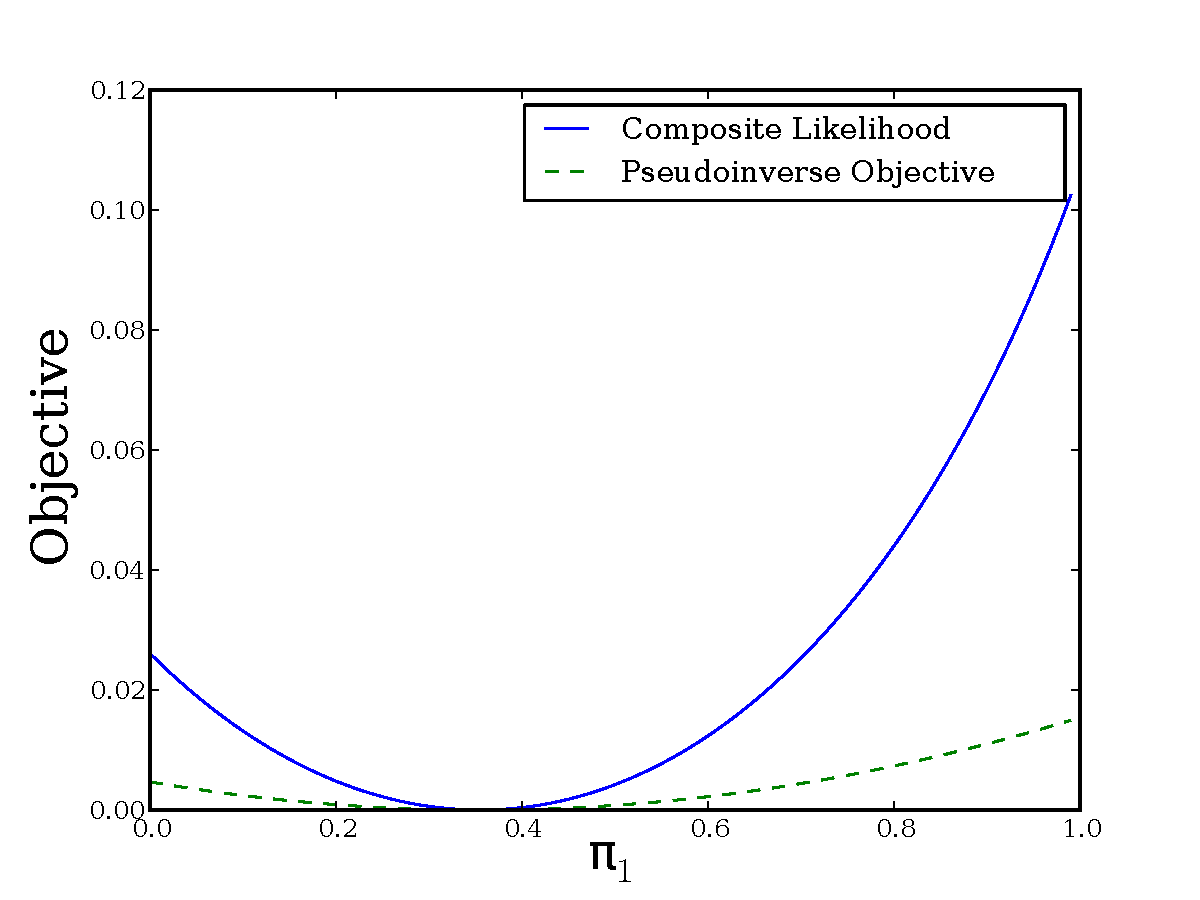
\includegraphics[width=0.45\columnwidth]{figures/piecewise-objective.pdf}
  %  }
%  \subfigure[Directed grid model] {
%    \label{fig:examples-grid}
%    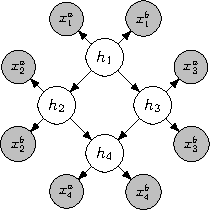
\includegraphics{figures/grid.pdf}
%  }
%  \subfigure[] {
  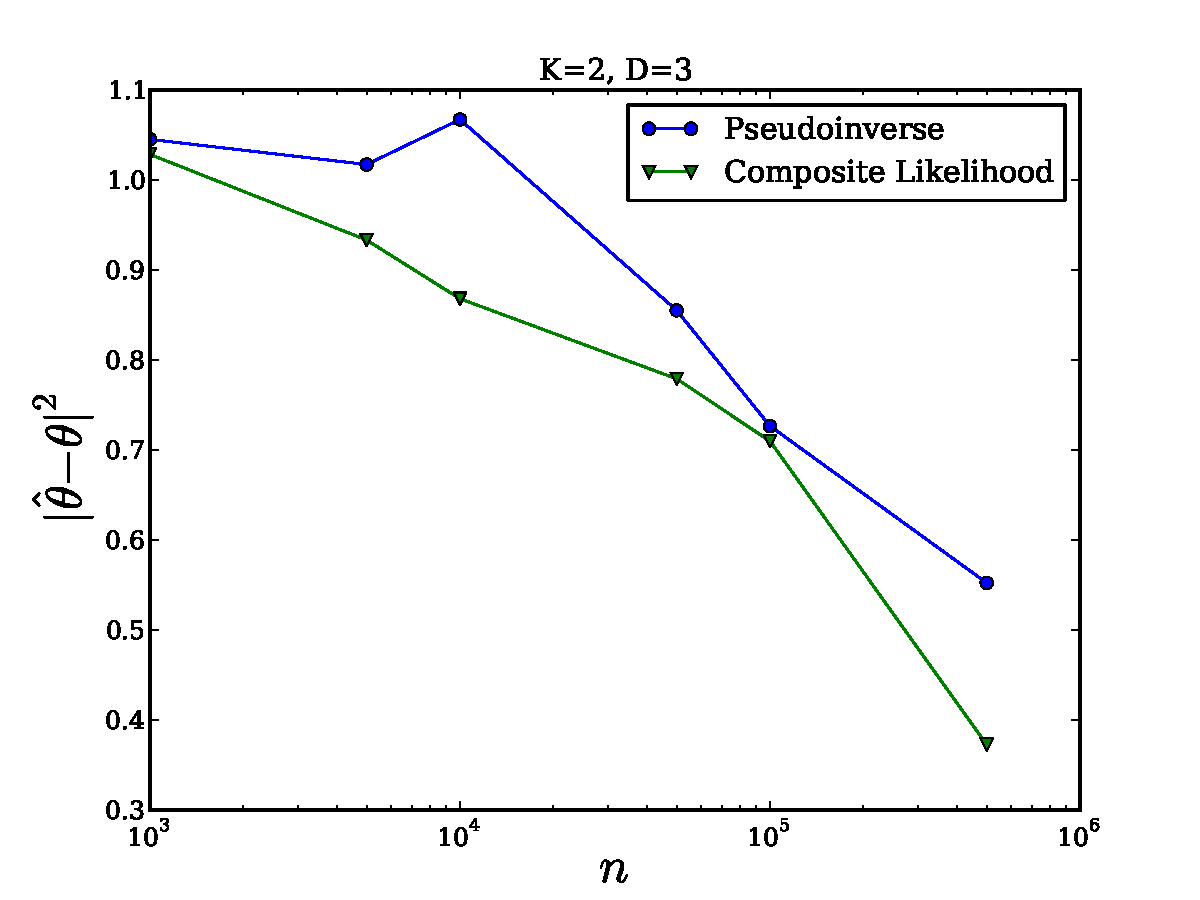
\includegraphics[width=0.8\columnwidth]{figures/hmm-2-3.pdf}
%  }
  \caption{Parameter estimation error when recovering parameters for a Hidden
  Markov Model with $k=2$ states and $d=3$ emissions using two types of estimators.}
    \label{fig:cl-hmm}
\end{figure}

\section{Parameter Estimation for Log-linear Latent-Variable Models}
\label{sec:log-linear}

\paragraph{Setup}
Let $z$ be a collection of variables indexed by $V$ (that is, $z = \{z_j\}_{j \in V}$).
Suppose that some of the variables are observed ($x = \{ z_j \}_{j \in O}$, where $O \subset V$) 
and the rest are hidden ($h = \{ z_j \}_{j \in H}$, where $H = V \backslash O$).
Let $C \subset 2^V$ be a collection of subsets of variables,
and let $\phi_c(z_c) \in \Re^d$ be the feature map for each $c \in C$.
In this paper, we will consider both directed and undirected models over $z$.
In the undirected case, we define the standard globally-normalized exponential family model:
\begin{align}
  \label{eqn:undirectedSetup}
  p_\theta(z) = \exp\{ \phi(z)^\top\theta - A(\theta) \},
\end{align}
where $\phi(z) \eqdef \sum_{c \in C} \phi_c(z_c) \in \Re^d$ is the global feature vector, $\theta \in \Re^d$ is the parameter vector,
and $A(\theta) = \log \int \exp\{\phi(z)^\top\theta\} dz$ is the global log-partition function.
To some extent, our methods only depend on the conditional independence
structure of the models.

\paragraph{Problem statement}

% Statement
This paper focuses on the problem of parameter estimation:
We are given $n$ i.i.d.~examples of the observed variables $D = (x^{(1)}, \dots, x^{(n)})$
where each $x^{(i)} \sim p_{\theta^*}$ for some true parameters $\theta^*$.
Our goal is to produce a parameter estimate $\hat\theta$ that approximates $\theta^*$.

% Maximum likelihood
The standard estimation procedure is maximum (marginal) likelihood,
$\sL \eqdef \max_{\theta \in \Re^d} \sum_{x \in D} \log p_\theta(x)$,
which is statistically efficient but computationally intractable.
In practice, one uses gradient-based optimization procedures (e.g., EM or L-BFGS)
on the marginal likelihood, which can get stuck in local optima.

\paragraph{Primer: Three-view log-linear mixture models}

\citet{anandkumar12moments} describe an algorithm to recover parameters
  for a directed three-view mixture model. 
We will consider an undirected log-linear model variant of this model,
  shown in \figureref{three-view}.
The model has features $\phi(x,y) = \{\bI(x_1,y_1), \bI(x_2,y_1), \bI(x_2,y_1)\}$.

Recover moments with tensor factorization.
Show that the constrained optimization problem is convex.

Statement: consistency.


\section{Experiments} \label{sec:experiments}

%We have argued the case for using measurements of the latent moments to 
%aid parameter estimation.
The spectral decomposition (Steps 1 and 2) in \refsec{threeViewMixtureModel}
provides measurements,
which are used in the optimization problem \refeqn{minKL}.
In this section, we
seek to answer two questions empirically:
(i) how much do the measurements aid estimation, and
(ii) how effectively are the measurements estimated using the
method of moments.
%We found that measurements can improve the fit of the
%parameters estimated considerably.
%While empirical measurements estimated using the
%method of moments are less accurate, we still find that they improve
%parameter estimates in general.

% Do measurements help in parameter estimation?
\paragraph{Measurements}

We generated 10 random hidden Markov models,
each with $k=3$ hidden states and $\ell=5$ possible observed values. 
For each model, we generated 10 sets of $n=10,000$ sequences of length $L=3$.
We compared the prediction accuracy of parameters estimated using EM
initialized using \refeqn{minKL} when different percentages of the expected
latent measurements, $\E[\phi(x,h)]$, were observed.

%For example, we ran one experiment where we assumed 10\% of the latent
%measurements were observed.

\Fig{figures/measurements}{0.3}{measurements}{a}

\reffig{measurements} shows the prediction error of the parameters
micro-averaged over the different data and models.  First, as we get more
measurements, prediction error decreases.  Second,
learning from only the emissions moments works comparably
to using emissions and transitions, verifying the fact that
we can get leverage from partial information.\footnote{
These numbers are high releative because they use empirical moments
whereas the curve is based on expected moments.}

%For comparison, we have
%included the accuracy achieved using the method of moments estimation procedure
%described in \refsec{factorization} with empirical moment estimates.  We see
%that using measurements for even a small percentage of features can improve
%prediction accuracy by \todo{x\%}. Spectral estimates too improve accuracy,
%though not as markedly; we observed a \todo{x\%} improvement.

% - we ran experiments with different proportions of the expected feature counts being observed and plot performance here. 
% - while such information is not available in practice, we note that it provides a significant improvement over learning with just EM.
% - next, we used spectral techniques to estimate the counts on the data and observed that it also showed a concrete improvement in performance, though not as much as the measurements.

% details:
% - For purposes of illustration, we looked at 10 different hmms with
% parameters $K=3$, $D=5$ and $N=10^5$ samples. We ran each experiment for
% 10 different data samples and report the micro-averages.

% Could it be effective in practice?
\paragraph{General results}

\begin{table}
    \label{tab:errors}
    \begin{tabular}{l | l l | l l l }
        Algorithm & $k$ & $d$ & Accuracy & $\Delta \hat \E[\phi(x,h)]$ & Log Likelihood \\ \hline
        & \multicolumn{2}{|c|}{Mixtures} & & & \\ \hline
        \multirow{3}{*}{EM} 
        & 3 & 2 & 0.65 (+/- 0.01) & 1.23 & -3.72 \\
        & 3 & 3 & 0.51 (+/- 0.06) & 1.81 & -4.21\\
        & 5 & 2 & 0.72 (+/- 0.07) & 1.13 & -5.21\\ \hline
        \multirow{3}{*}{Spectral} 
        & 3 & 2 & 0.80 (+/- 0.09) & 0.23 & -3.54 \\
        & 3 & 3 & 0.68 (+/- 0.10) & 1.01 & -3.76 \\
        & 5 & 2 & 0.80 (+/- 0.05) & 0.18 & -5.04 \\ \hline
        \multirow{3}{*}{100\% Measurements} 
        & 3 & 2 & 0.80 (+/- 0.08) & 0.01& -3.54 \\
        & 3 & 3 & 0.70 (+/- 0.11) & 0.02& -3.87 \\
        & 5 & 2 & 0.80 (+/- 0.05) & 0.01& -5.03 \\ \hline
        & \multicolumn{2}{|c|}{HMMs} & & & \\ \hline
        \multirow{3}{*}{EM} 
& 3 & 2 & 0.64 (+/- 0.10) & 1.71 & -4.51 \\  
& 3 & 3 & 0.42 (+/- 0.05) & 2.41 & -6.09 \\  
& 5 & 2 & 0.62 (+/- 0.09) & 1.60 & -6.47 \\  \hline
        \multirow{3}{*}{Spectral} 
& 3 & 2 & 0.67 (+/- 0.07) & 2.59 & -3.71 \\ 
& 3 & 3 & 0.45 (+/- 0.08) & 4.96 & -4.36 \\ 
& 5 & 2 & 0.64 (+/- 0.10) & 3.43 & -5.31 \\ \hline
        \multirow{3}{*}{100\% Measurements} 
& 3 & 2 & 0.71 (+/- 0.07) & 0.39 & -4.64 \\ 
& 3 & 3 & 0.47 (+/- 0.07) & 1.53 & -5.85 \\ 
& 5 & 2 & 0.73 (+/- 0.07) & 0.39 & -6.16 \\ \hline
    \end{tabular}
    \caption{Micro-averaged Errors.}
\end{table}

%Having shown that measurements can help the task of parameter estimation, we
\reftab{errors} shows results for the mixture model and HMM.
For each row, we report prediction accuracy
over 5 different models with the specified number of parameters and 5 random
samples of $10,000$ instances from the model. 
We see that using measurements recovered from spectral decomposition
helps significantly over EM, sometimes matching
using the true expected measurements.

%In the table, we compare randomly initialized EM with EM initialized using (a)
%empirical measurements estimated with the method of moments and (b) fully
%expected measurements.

First, we note that we found measurements to uniformly improve the prediction
accuracy of EM. The picture for method of moments is similar, though there is
greater variation in the improvement it provides.

% - Generated data from different 3-view mixture models and hmms. 
% - Each averages over 5 different parameters and 5 different data samples.
% - Find that there is quite some variation in spectral performance, but measurements uniformly helps estimation.

% \subsection{Basic mixture model}
% 
% Show simple mixture model works on artifical data.
% 
% Show EM/gradient gets stuck in local optima.
% 
% spectral methods are not statistically efficient (especially with parameter sharing).
% 
% \subsection{Measurements}
% 
% For models in \reffig{generalModels}, do experiments.
% 
% Show that the non-convexity decreases.
% 
% \subsection{Factorial models}
% 
% Show that the unshuffling basically works with near infinite data, while EM gets stuck in local optima.
% 
% \subsection{Part-of-speech induction}
% 
% \cite{kirkpatrick10painless} trains for 1,000 iterations, which takes a long time.
% 63.1\% Basic HMM
% 68.1\% EM, L-BFGS 75.5\%
% 
% Can we match the performance?
% 
% Also, since method of moments doesn't require inference, can we use a much larger corpus
% and get better results.

\section{Conclusion}
\label{sec:conclusion}



\bibliography{pliang}
\bibliographystyle{icml2014}

\end{document} 

